% -*- Mode:TeX -*-

%% IMPORTANT: The official thesis specifications are available at:
%%            http://libraries.mit.edu/archives/thesis-specs/
%%
%%            Please verify your thesis' formatting and copyright
%%            assignment before submission.  If you notice any
%%            discrepancies between these templates and the 
%%            MIT Libraries' specs, please let us know
%%            by e-mailing thesis@mit.edu

%% The documentclass options along with the pagestyle can be used to generate
%% a technical report, a draft copy, or a regular thesis.  You may need to
%% re-specify the pagestyle after you \include  cover.tex.  For more
%% information, see the first few lines of mitthesis.cls. 

%\documentclass[12pt,vi,twoside]{mitthesis}
%%
%%  If you want your thesis copyright to you instead of MIT, use the
%%  ``vi'' option, as above.
%%
%\documentclass[12pt,twoside,leftblank]{mitthesis}
%%
%% If you want blank pages before new chapters to be labelled ``This
%% Page Intentionally Left Blank'', use the ``leftblank'' option, as
%% above. 

\documentclass[12pt,twoside]{mitthesis}
\usepackage{lgrind}
%% These have been added at the request of the MIT Libraries, because
%% some PDF conversions mess up the ligatures.  -LB, 1/22/2014
\usepackage{cmap}
\usepackage{amsmath}
\usepackage[T1]{fontenc}
\usepackage{graphicx}
\usepackage{subcaption}
\graphicspath{ {./images/} }
% Added by me - makes the TOC into hyperlinks
\usepackage{color}
\usepackage{hyperref}
\hypersetup{
    colorlinks,
    citecolor=blue,
    filecolor=black,
    linkcolor=blue,
    urlcolor=blue
}

\pagestyle{plain}


%% This bit allows you to either specify only the files which you wish to
%% process, or `all' to process all files which you \include.
%% Krishna Sethuraman (1990).

\begin{document}
\pagestyle{plain}

\begin{flushright}
William Cook\\
Machine Learning\\
Final Project\\
Due 12/14/2018\\
\end{flushright}

\section{Abstract}

The \textbf{daWUAP} team at the University of Montana has created a hydrological rainfall-runoff model that predicts streamflows across the state of Montana. \textbf{daWUAPhydroengine} is informed by a variety of smaller models, including a groundwater model, snow water equivalient (swe) model, and agricultural component model. Despite this complexity, \textbf{daWUAPhydroengine} is designed to be a quick and efficient model.

This paper focuses on the calibration of \textbf{daWUAPhydroengine} via a Dual State Parameter Estimation Ensemble Kalman Filter. Uniquely, this filter operates on multiple high dimensional parameters represented as raster images. These raster images are both ingested and outputted by the \textbf{daWUAPhydroengine} and were previously set at a constant value. The filter aims to both calibrate and distribute these variables geospatially. 

  % -*- Mode:TeX -*-
%% This file simply contains the commands that actually generate the table of
%% contents and lists of figures and tables.  You can omit any or all of
%% these files by simply taking out the appropriate command.  For more
%% information on these files, see appendix C.3.3 of the LaTeX manual. 
\tableofcontents
\addcontentsline{toc}{chapter}{Symbols}
\newpage
\listoffigures
\newpage
\listoftables


\chapter{Introduction}



	Utilizing sequential data assimilation techniques to filter hydrologic models is an efficient way to correct and calibrate them both before and after implementation in the field. Many observations such as SWE, streamflow, and precipitation are collected on a daily basis across various geographic regions, allowing the previous day's information to be dynamically ingested by the hydrologic model and inform current predictions. These models allow hydrologists to understand the past and predict the future.
	
	Models that ingest data sequentially can be efficiently corrected by a Kalman Filter, a sequential data assimilation algorithm. Kalman Filters only need the previous timestep's state estimate, parameter estimate, and co-variance matrices to update the current timestep's state estimate, parameter estimate, and co-variance matrices. However, the original Kalman filter\cite{Kalman1960} was created to solve linear problems, and more complicated implementations must be used to solve non-linear problems. The extended Kalman Filter\cite{Jazwinski1970} works for mildly non-linear systems but does not function optimally on heavily non-linear systems\cite{Miller1994}. The Unscented Kalman Filter\cite{Julier1997} is an all-around improvement on the Extended Kalman Filter that allows for the filtering of highly non-linear systems. The Ensemble Kalman Filter\cite{Evensen1994}, a predecessor to the Unscented Kalman Filter, filters non-linear systems by generating an 'ensemble' of model instances and adding unique noise to each model's forcing data. The main advantage of this ensemble based approach is the substitution of the original Kalman Filter's error covarience matrix with an ensemble covariance matrix, which allows for the efficient computation of the covariance of high dimensional state vectors. 
	
	In order to calibrate parameters within a hydrologic model a Dual State Kalman Filter may be used. Dual state Kalman filters add a small perturbation to a series of parameters that the use rwishes to calibrate. These perturbed parameters vectors are then corrected in a similar fashion to the state vectors. After this happens a 'second' filter runs and corrects the state vectors in the normal fashion. The Dual State Ensemble Kalman Filter implemented by Moradkhani et. al\cite{Moradkhani2005} extends the Ensemble Kalman Filter into a dual state configuration.
	
	 To examines the Dual State Ensemble Kalman Filter's application to high dimensional geospatially distributed raster data Professor Marko Maneta's \textbf{daWUAPhydroengine} is used. Professor Maneta and his team have created a hydrological rainfall-runoff model that predicts streamflows across the state of Montana. \textbf{daWUAPhydroengine} is informed by a variety of smaller models, including a groundwater model, snow water equivalient (swe) model, and agricultural component model. Despite this complexity, \textbf{daWUAPhydroengine} is designed to be a quick and efficient model. \textbf{daWUAPhydroengine} is influenced by a series of uncalibrated high-dimensional parameters that are stored as 2D raster data. A Dual Ensemble Kalman Filter is an optimal calibration algorithm to calibrate this raster data because 1) the DEnKF does not have to compute the high dimensional state covariance matrix and 2) \textbf{daWUAPhydroengine} is a sequential model.
	
	Chapter 2 covers the methods behind the Dual Ensemble Kalman Filtering algorithm originally implemented by Moradkhani et al. Chapter 3 displays results of applying the Dual State Kalman Filter to \textbf{daWUAPhydroengine}. Chapter 4 discusses improvements currently being made, particularly the plans for a new, innovative hierarchical algorithm.
	
	
	

	
%% This is an example first chapter.  You should put chapter/appendix that you
%% write into a separate file, and add a line \include{yourfilename} to
%% main.tex, where `yourfilename.tex' is the name of the chapter/appendix file.
%% You can process specific files by typing their names in at the 
%% \files=
%% prompt when you run the file main.tex through LaTeX.
\chapter{Theory}



\section{The History of Kalman Filters}

R.E Kalman published the article \textit{A New Approach to Linear Filtering and Prediction Problems} in 1960 \cite{Kalman1960}. Since then, the so-called "Kalman Filter" has been tested, researched, and improved extensively. Kalman's original algorithm was limited to linear systems. The development of the Extended Kalman Filter allowed Kalman Filters to operate on non-linear systems with some limitations. More recently, the Unscented Kalman Filter \cite{Julier1997} and the Ensemble Kalman Filter \cite{Evensen1994} have been developed to work on non-linear systems.

\section{The Linear Kalman Filter}

The original Kalman filter was created to solve problems where both a predictive sequential model and a series of observations is available. The predictive model can be represented as the linear stochastic difference equation
\begin{large}
\begin{equation}\label{eq:2p1}
x_{i} = Ax_{i-1} + Bu_{i-1} + w_{i-1}
\end{equation}
\end{large}

Where $A$ is the model matrix which serves to transform the vector $x_{i-1}$ to the current timestep, $B$ is the control matrix that transforms the control vector $u_{i}$ to account for external forces on the model, $w_{i}$ is a vector of model error, and $i$ is the timestep.

An observation for any given timestep $i$ can be represented as 

\begin{large}
\begin{equation}\label{eq:2p2}
z_{i} = Hx_{i} + v_{i}
\end{equation}
\end{large}

where $z_{i}$ is the vector of observations, $x_{i}$ is the vector of true states, $H$ is a masking matrix, and $v_{i}$ is a vector of measurement errors. $w_{i}$ and $v_{i}$ are assumed to be independent, normally distributed random variables with probability distributions defined by

\begin{large}
\begin{equation}\label{eq:2p3}
P(w) \sim N(0,Q)
\end{equation}
\begin{equation}\label{eq:2p4}
P(v) \sim N(0,R)
\end{equation}
\end{large}

\subsection{Algorithm}

Kalman filters optimize model predictions by blending predicted states with that timestep's observations. Conveniently, the algorithm's steps are separated into \textit{prediction} and \textit{update} categories. The initial prediction algorithm \eqref{eq:2p5} obtains the current timestep's vector of states using the same equation as \eqref{eq:2p1} with the removal of the random unknown vector $w$. To track the effects of ignoring $w$ the prior error covariance matrix $P^{-}$ is calculated \eqref{eq:2p6}.

\begin{table}[h]
\caption{Prediction Equations - Discrete Kalman Filter} 
\centering
\begin{tabular}{c c}
\\ [0.1ex] 
\hline   
Name & Equation \\
\hline
Model Prediction & \parbox{3cm}{\begin{equation}\label{eq:2p5} \hat{x}^{-}_{i} = A\hat{x}^{+}_{i-1} + Bu_{i-1} \end{equation}} \\
Update Prior Covariance & \parbox{3cm}{\begin{equation}\label{eq:2p6} P^{-}_{i} = AP^{+}_{i}A^{T}+Q \end{equation}}
\end{tabular}
\label{tab:hresult}
\end{table}

Equation \eqref{eq:2p8} returns the updated prediction $\hat{x}^{+}_{i}$ by multiplying the innovation between the observation and the masked prediction by the kalman gain $K$, which is defined in \eqref{eq:2p7}. Finally, the error covariance matrix is updated in \eqref{eq:2p9} to reflect the more accurate nature of the updated prediction.

\begin{table}[h]
\caption{Update Equations - Discrete Kalman Filter} 
\centering
\begin{tabular}{c c}
\\ [0.1ex]
\hline
Name & Equation \\ [0.5ex]
\hline            
Kalman Gain & \parbox{3cm}{\begin{equation}\label{eq:2p7}K_{i} = P^{-}_{i}H^{T}(HP^{-}_{i}H^{T} + R)^{-1} \end{equation}} \\
Update Estimate & \parbox{3cm}{\begin{equation}\label{eq:2p8} \hat{x}^{+}_{i} = \hat{x}^{-}_{i} + K_{i}(z_{i}-H\hat{x}_{i}) \end{equation}} \\
Update Posterior Covariance & \parbox{3cm}{\begin{equation}\label{eq:2p9}P^{+}_{i} = (I-K_{i}H)P^{-}_{i} \end{equation}}
\end{tabular}
\label{tab:hresult}
\end{table}


\section{The Dual Ensemble Kalman Filter}

According to Jazwinski \cite{Jazwinski1970} any discrete nonlinear stochastic-dynamic model can be defined as:

\begin{equation}\label{eq:gen_stoc}
x_{t+1} = f(x_{t}, u_{t}, \theta_{t}) + \varepsilon_{t}
\end{equation}

where $x_{t}$ is an $n$ dimensional vector representing the state variables of the model at time step $t$, $u_{t}$ is a vector of forcing data (e.g temperature or precipitation) at time step $t$, and $\theta_{t}$ is a vector of model parameters which may or may not change per time step (e.g \textit{soil beta }or \textit{DDF}). The non-linear function $f$ takes these variables as inputs. The noise variable $\varepsilon_{t}$ accounts for both model structural error and for any uncertainty in the forcing data.

A state's observation vector $z_{t}$ can be defined as

\begin{equation}\label{eq:gen_obs}
z_{t} = h(x_{t}, \theta_{t}) + \delta_{t}
\end{equation}

Where the $x_{t}$ vector represents the true state, $\theta_{t}$ represents the true parameters, $h(.)$ is a function that determines the relationship between observation and state vectors, and $\delta_{t}$ represents observation error. $\delta_{t}$ is Gaussian and independent of $\varepsilon_{t}$.

The Dual State Ensemble Kalman Filter can be split into three subsections: The prediction phase, the parameter correction phase, and the state correction phase. 

\subsection{Prediction Phase}

In a Dual Ensemble Kalman filter, each ensemble member \textit{i} is represented by a stochastic model similar to \eqref{eq:gen_stoc}. The modified equation is as follows:

\begin{equation}\label{eq:dekf_predict}
x_{t+1}^{i-} = f(x_{t}^{i+}, u_{t}^{i}, \theta^{i-}_{t}) + \omega_{t}, \quad i=1,...,n
\end{equation}

Where $n$ is the total number of ensembles. The $-/+$ superscripts denote corrected ($+$) and uncorrected ($-$) values. Note that $\theta^{i-}_{t}$'s $t$ superscript does not necessarily denote that $\theta$ is time variant but rather indicates that parameter values change as they are filtered over time. The noise term $\omega_{t}$ accounts for model error and will hereafter be excluded from the state equation.

Errors in the forcing data are accounted for through the perturbation the forcing data vector $u_{t}$ with random noise $\zeta_{t}^{i}$ to generate a unique variable $u_{t}^{i}$ for each ensemble. $\zeta_{t}^{i}$ is drawn from a normal distribution with a covarience matrix $Q_{t}^{i}$.

\begin{equation}\label{eq:dekf_u}
u_{t+1}^{i} = u_{t} + \zeta_{t}^{i}, \quad \zeta_{t}^{i} \sim N(0,Q_{t}^{i}) 
\end{equation}

To generate the priori parameters $\theta^{i-}_{t+1}$ an evolution of the parameters similar to the evolution of the state variables must be implemented. To accomplish this the kernel smoothing technique developed by West\cite{West1993} and implemented by Liu \cite{Liu2000} is used. Legacy implementations of parameter evolution added a small perturbation sampled from $N(0,\Sigma^{\theta}_{t})$, where $\Sigma^{\theta}_{t}$ represents the covariance matrix of $\theta$ at timestep $t$. This legacy method of evolution resulted in overly disposed parameter samples and the loss of continuity between two consecutive points in time \cite{Liu2000} \cite{Chen2008}. Kernel smoothing has been used effectively to solve this problem in previous Dual Ensemble Kalman filter implementations \cite{Moradkhani2005} and similar models \cite{Chen2008}.

\begin{equation}\label{eq:dekf_thetaminus}
\theta_{t+1}^{i-} = a\theta_{t}^{i+} + (1-a)\bar{\theta}_{t}^{+} + \tau_{t}^{i}
\end{equation}
\begin{equation}\label{eq:dekf_tau}
\tau_{t}^{i} = N(0, h^{2}V_{t})
\end{equation}
 
Where $\bar{\theta}_{t}^{+}$ is the mean of the parameters with respect to the ensembles, $V_{t} = var(\theta_{t}^{i+})$, $a$ is a shrinkage factor between (0,1) of the kernel location, and $h$ is a smoothing factor. $h$ is defined by $\sqrt{1-a1/2}$, while $a$ is generally between (.45,.49). Note that $h$ and $a$ tend to vary per model and optimal values for these parameters are generally found via experimentation  \cite{Moradkhani2005}  \cite{Anderson1999} \cite{Annan2005} \cite{Chen2008}.

\subsection{Parameter Correction Phase}

In an Ensemble Kalman Filter, observations are perturbed to reflect model error. Therefore, the variable $z_{t+1}^{i}$ is defined as follows:

\begin{equation}\label{eq:dekf_obs}
z_{t+1}^{i} = z_{t+1} + \eta_{t+1}^{i},\quad \eta_{t+1}^{i} = N(0,R_{t+1})
\end{equation}

Where $z_{t+1}$ is an observation vector defined by \eqref{eq:gen_obs} and $\eta_{t+1}^{i}$ is a random perturbation drawn from a normal distribution with covarience matrix $R_{t+1}$. A set of state predictions that can be related to the observations are generated by running the priori state vector through the function $h(.)$:

\begin{equation}\label{eq:dekf_pred}
\hat{y}_{t+1}^{i} = h(x_{t+1}^{i-}, \theta_{t+1}^{i-})
\end{equation}

The parameter update equation is similar to the update equation of the linear Kalman filter ($\hat{x}^{+}_{t} = \hat{x}^{-}_{t} + K_{t}(z_{t}-H\hat{x}_{t})$) Notably,  parameters are corrected in lieu of the states:

\begin{equation}\label{eq:dekf_param_update}
\theta_{t+1}^{i+} = \theta_{t+1}^{i-} + K_{t+1}^{\theta}(z_{t+1}^{i}-\hat{y}_{t+1}^{i})
\end{equation}

To facilitate this, $K_{t+1}^{\theta}$ is defined as

\begin{equation}\label{eq:dekf_param_k}
K_{t+1}^{\theta} = \frac{\Sigma^{\theta,\hat{y}}_{t+1}}{\Sigma^{\hat{y},\hat{y}}_{t+1} + R_{t+1}}
\end{equation}

where $\Sigma^{\theta,\hat{y}}_{t+1}$ is the cross covariance of $\theta_{t+1}$ and $\hat{y}_{t+1}$, $\Sigma^{\hat{y},\hat{y}}_{t+1}$ is the covarience of $\hat{y}_{t+1}$, and $R_{t+1}$ is the observation error matrix from \eqref{eq:dekf_obs}. 

\subsection{State Correction Phase}

After $\theta_{t+1}^{i+}$ has been calculated the model is run again \eqref{eq:dekf_predict} with the $\theta_{t+1}^{i+}$ replacing $\theta_{t+1}^{i-}$.

\begin{equation}\label{eq:dekf_predict_2}
x_{t+1}^{i-} = f(x_{t}^{i+}, u_{t}^{i}, \theta^{i+}_{t}), \quad i=1,...,n
\end{equation}

After a new state vector is generated it is re-run through \eqref{eq:dekf_pred} with the new parameter vector:

\begin{equation}\label{eq:dekf_pred_2}
\hat{y}_{t+1}^{i} = h(x_{t+1}^{i-}, \theta_{t+1}^{i+})
\end{equation}

The corrected state vector is then run through the state update equation

\begin{equation}\label{eq:dekf_state_update}
x_{t+1}^{i+} = x_{t+1}^{i-} + K_{t+1}^{x}(z_{t+1}^{i}-\hat{y}_{t+1}^{i})
\end{equation}
 
\begin{equation}\label{eq:dekf_param_k}
K_{t+1}^{x} = \frac{\Sigma^{x,\hat{y}}_{t+1}}{\Sigma^{\hat{y},\hat{y}}_{t+1} + R_{t+1}}
\end{equation}

where $\Sigma^{x,\hat{y}}_{t+1}$ is the cross covariance of $x_{t+1}$ and $\hat{y}_{t+1}$.




%% This is an example first chapter.  You should put chapter/appendix that you
%% write into a separate file, and add a line \include{yourfilename} to
%% main.tex, where `yourfilename.tex' is the name of the chapter/appendix file.
%% You can process specific files by typing their names in at the 
%% \files=
%% prompt when you run the file main.tex through LaTeX.
\chapter{Application of DEnHKF to Hydrologic Model}

\section{daWUAPhydroengine}

The \textbf{daWUAPhydroengine} hydrologic dynamic model is used to test the viability of the DEnHKF method.  \textbf{daWUAPhydroengine} takes streamflow and subbasin parameters, precipitation, minimum temperatures, and maximum temperatures as inputs and outputs streamflow data along with some additional states such as snow water equivalent. \textbf{daWUAPhydroengine} was designed to be implemented in any geographic location. For this study it was utilized to model streamflows throughout the state of Montana.

\begin{table}[]
\caption{States} 
\begin{tabular}{lll}
State ($x$) & Purpose                              & Dimensions  \\ \hline
streamflow  & Streamflow (in cumecs)               & 330   \\
swe         & Snow Water Equivalent  (in $mm^{3}$) & 45012
\end{tabular}
\label{tab:states}
\end{table}

Configuring \textbf{daWUAPhydroengine} to model streamflows throughout Montana is advantageous because it allows for the calibration of a very large number of spatially distributed, high dimensional parameters. These parameters span the entirety of Montana, which covers an area of 380,800 $km^{2}$. Montana's large geographical coverage is diverse and the terrain differs in various ways (soil composition, forestation, etc.)

\begin{table}[]
\caption{Forcing Data} 
\begin{tabular}{lll}
Forcing Data ($u$) & Purpose                          & Dimensions \\ \hline
tempmin          & Lowest temperature for timestep  & 45012 \\
tempmax          & Highest temperature for timestep & 45012 \\
precipitation      & Amount of rainfall for timestep & 45012 
\end{tabular}
\label{tab:u_params}
\end{table}

\begin{table}[]
\caption{Calibrated Parameters} 
\begin{tabular}{lll}
Parameter ($\theta$) & Purpose                                                    & Dimensions  \\ \hline
ddf                  & Controls Rate of Snowfall                                        & 45012 \\
aet\_lp              & Controls AET                                                      & 45012 \\
soil\_beta           & Controls portion of ponded water that goes into soil storage & 45012 \\
soil\_max\_wat       & Controls soil maximum water capacity & 45012
\end{tabular}
\label{tab:t_params}
\end{table}

\begin{figure}[h]
    \centering
    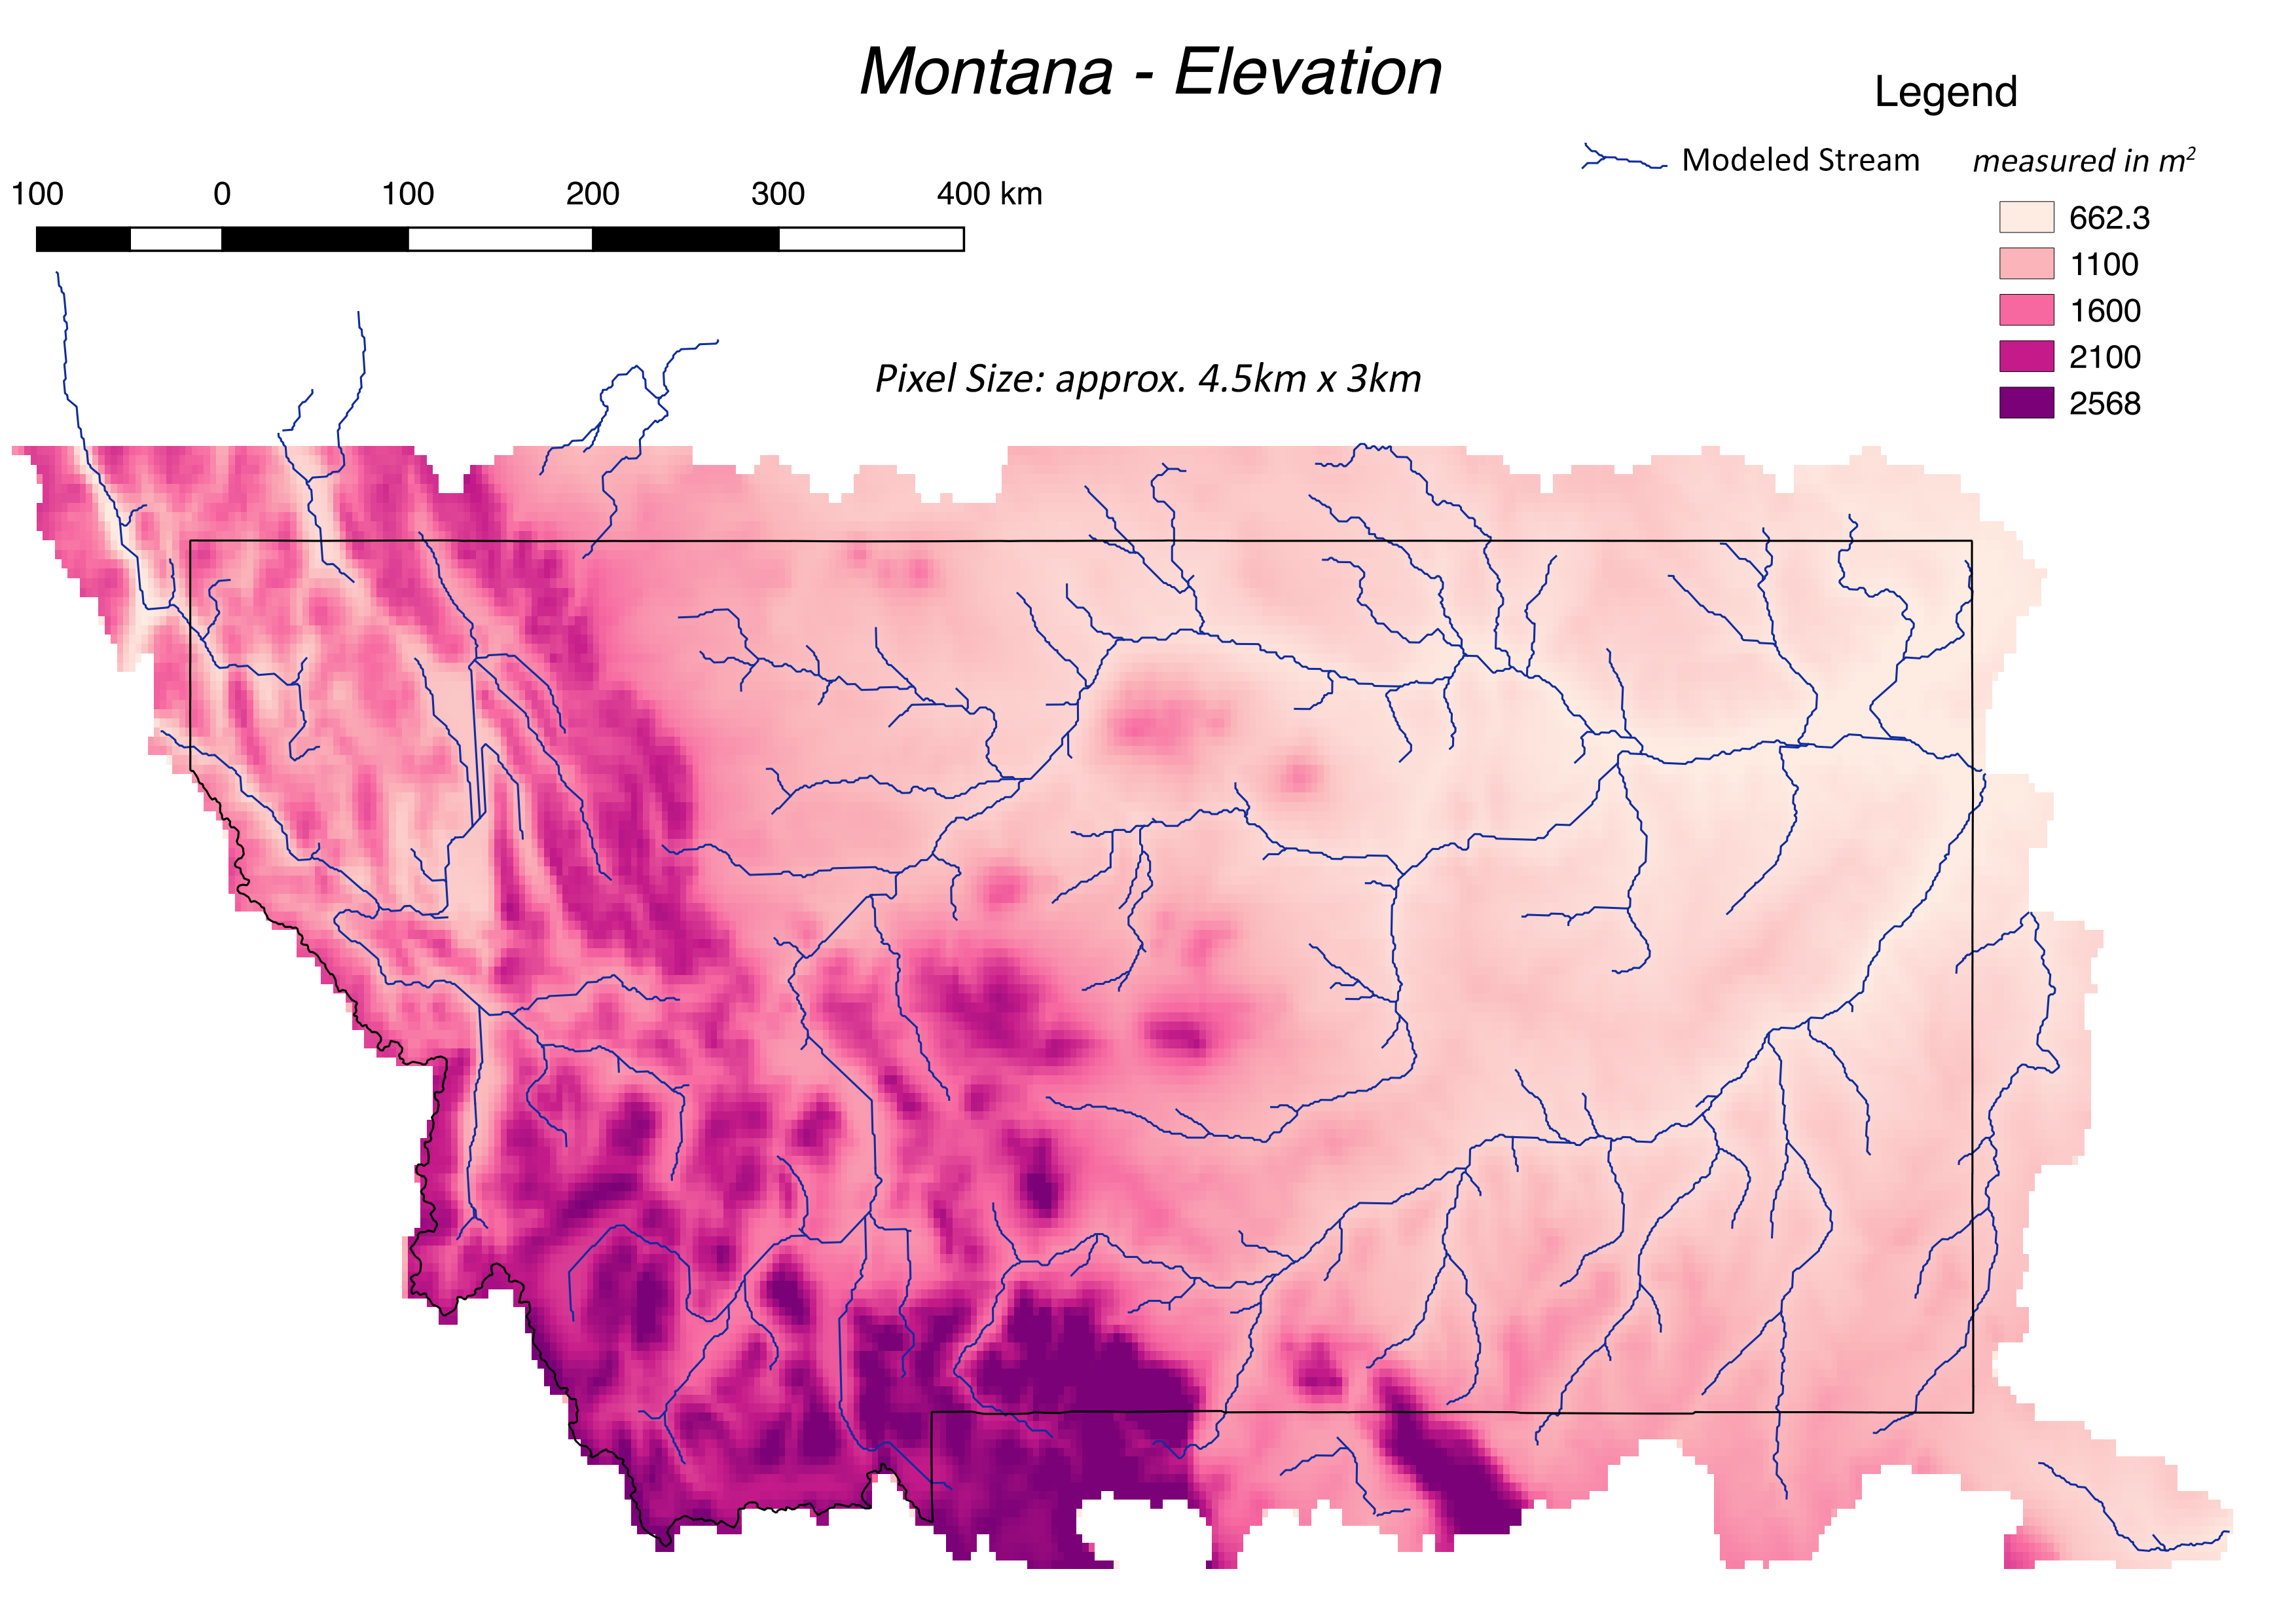
\includegraphics[width=0.95\textwidth]{elevation}
    \caption{Elevation throughout Montana}
    \label{fig:elevation}
\end{figure}

\section{Observation Data}

A Kalman Filter relies on one or more observed states for correction. Accordingly, observations were obtained for streamflows across Montana and snowfall across Montana. For streamflow, USGS streamflow data was collected at 86 sites. Each observed site was paired with the closest simulated \textbf{daWUAPhydroengine} stream outlet within a 2.5 mile cutoff. For snowfall, SNOWTEL sites monitored by the Natural Resources Conservation Service (NRCS) were used. 90 stations were chosen and matched to specific pixels in \textbf{daWUAPhydroengine}'s raster files.


\begin{table}[]
\caption{Observations} 
\begin{tabular}{lll}
Observed State ($x$) & Source                              & Dimensions  \\ \hline
streamflow  & USGS & 82   \\
swe         & NRCS & 90
\end{tabular}
\label{tab:obs}
\end{table}

\begin{figure}[h]
    \centering
    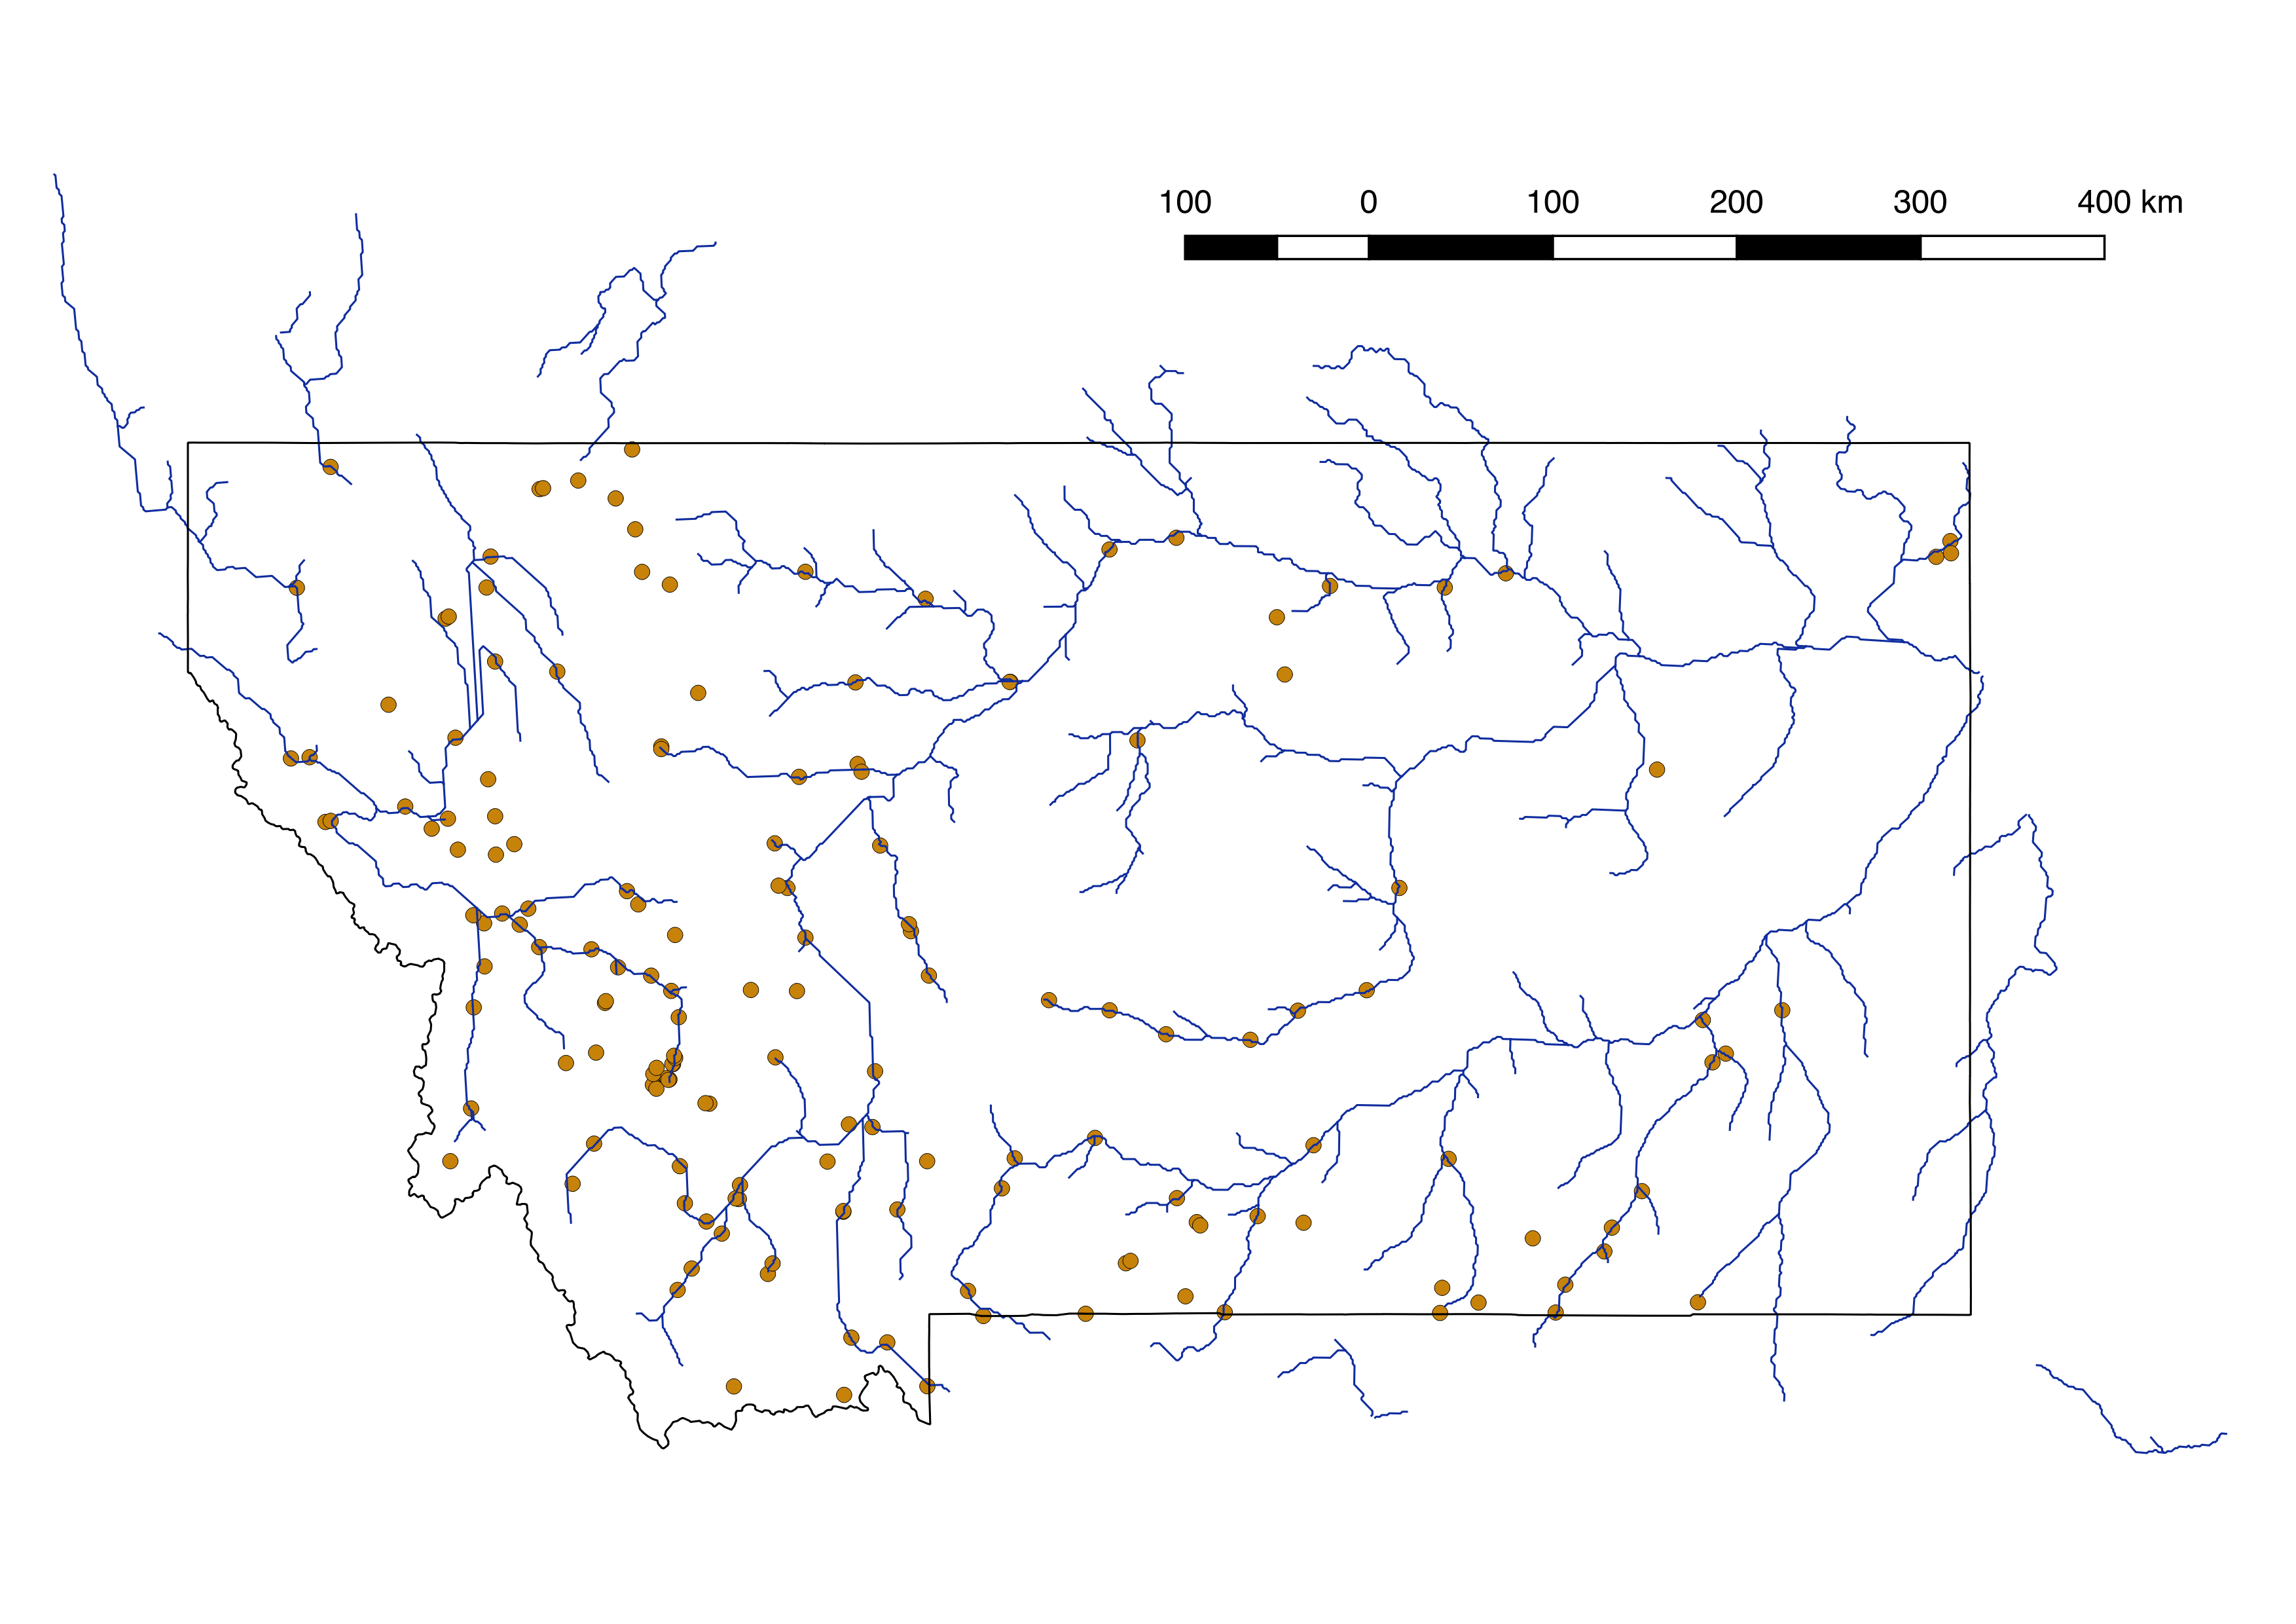
\includegraphics[width=0.95\textwidth]{stations}
    \caption{all SWE stations plotted against modeled streamflows}
    \label{fig:stations}
\end{figure}
%% This is an example first chapter.  You should put chapter/appendix that you
%% write into a separate file, and add a line \include{yourfilename} to
%% main.tex, where `yourfilename.tex' is the name of the chapter/appendix file.
%% You can process specific files by typing their names in at the 
%% \files=
%% prompt when you run the file main.tex through LaTeX.
\chapter{Discussion}

Currently, Prof. Johnson and Prof. Maneta and I are working on a way to combine a Hierarchical regression techinique with this Kalman filter. We believe that this will allow us to switch from the interpolation scheme shown earlier in this paper to a scheme where catchments are used as parameter zones.

\section{Hierarchical Kalman Filter}

The old equation for the evolution of priori parameters is:

\begin{equation}\label{eq:dekf_thetaminus}
\theta_{t+1}^{i-} = a\theta_{t}^{i+} + (1-a)\bar{\theta}_{t}^{+} + \tau_{t}^{i}
\end{equation}
\begin{equation}\label{eq:dekf_tau}
\tau_{t}^{i} = N(0, h^{2}V_{t})
\end{equation}
\begin{equation}\label{eq:dekf_V}
V_{t} = var(\theta_{t+1})
\end{equation}

Here is a draft of the hierarchical evolution:

\begin{equation}\label{eq:dekf_thetanew}
\theta_{t+1}^{i-} = \alpha_{t}^{i-}C_{t}^{i} + (1-\alpha_{t}^{i-})G_{t}^{i} + \tau_{t}^{i}
\end{equation}
\begin{equation}
C_{t}^{i} = a\theta_{t}^{i+} + (1-a)\bar{\theta}_{t}^{+}
\end{equation}
\begin{equation}
G_{t}^{i} = a \bar{\theta}_{t}^{i+} + (1-a)\bar{\bar{\theta}}_{t}^{+}
\end{equation}

\begin{equation}\label{eq:dekf_tau_2}
\tau_{t}^{i} = N(0, h^{2}V_{t})
\end{equation}

\begin{equation}\label{eq:dekf_V_2}
V_{t} = \alpha_{t}^{i-} var(h^{2}\theta_{t+1}) + (1-\alpha_{t}^{i-}) var(h^{2}G_{t}^{i})
\end{equation}
\begin{equation}\label{eq:dekf_V_3}
\alpha_{t+1}^{i-} = a\alpha_{t}^{i+} + (1-a)\bar{\alpha}_{t}^{+} + \delta_{t}^{i}
\end{equation}
\begin{equation}\label{eq:dekf_V_4}
\delta_{t} = N(0, h^{2}{}_{\alpha}V_{t})
\end{equation}
\begin{equation}\label{eq:dekf_V_5}
{}_{\alpha}V_{t} = var(\alpha_{t})
\end{equation}

Where initial $\alpha$, $m$, and $n$ are variables choosable by the user. This is a work in progress.


\chapter{Conclusion}

In conclusion, this Dual Ensemble Kalman Filter was sucessfully implemented on a hydrologic model. The resulting parameters do lead to better estimation of hydrologic components. Although these results are good, we hope to eventually implement an innovative new Hierarchical Kalman filter that will calibrate parameters at the catchment level.


\appendix
%% This defines the bibliography file (main.bib) and the bibliography style.
%% If you want to create a bibliography file by hand, change the contents of
%% this file to a `thebibliography' environment.  For more information 
%% see section 4.3 of the LaTeX manual.
\begin{singlespace}
\bibliography{main}
\bibliographystyle{plain}
\end{singlespace}

\end{document}

